\documentclass[conf]{new-aiaa}
%\documentclass[journal]{new-aiaa} for journal papers
\usepackage[utf8]{inputenc}

\usepackage{graphicx}
\usepackage{amsmath}
\usepackage{nomencl}
\usepackage[version=4]{mhchem}
\usepackage{siunitx}
\usepackage{longtable,tabularx}
\usepackage{float}
\setlength\LTleft{0pt} 

\title{Nintendo Wii Remote-Controlled Graphical User Interface for CrazyFlie Drone}

\author{Erika N. Jarosch\footnote{Student}, George V. Petrov\footnote{Student}, Justin L. Roskamp\footnote{Student}, and Kenneth T. Tochihara\footnote{Student}}
\affil{University of Illinois at Urbana-Champaign, Urbana, IL, 61820}

\begin{document}

\maketitle
\makenomenclature

% Erika
\begin{abstract} 
    The goal of this project is to design and implement a control interface between a Nintendo Wii remote and a Crazyflie 2.0 drone. The remote serves as an input device to a Windows device via a custom driver called HID WiiMote and emulates key and mouse inputs using JoyToKey. This input is then used with Python package Tkinter to convert Wii remote inputs to positional inputs, which can then be passed through the graphical user interface (GUI). The program interprets the positional inputs and then passes the translated flight plan to the Crazyflie via the input structures developed in the AE 483 course at the University of Illinois at Urbana-Champaign. This goal is motivated by the desire to use accessible platforms to inspire others with innovative and interactive aerobatics.

\end{abstract}

\mbox{}
\nomenclature{\( X_{Flight} =\)}{ The coordinate set, pixels }
\nomenclature{\( X_{World} =\)}{ The coordinate set, meters }
\nomenclature{\( W_{Canvas} =\)}{ The width of the square GUI drawing canvas, pixels}
\nomenclature{\( Zone =\)}{ The width of the Flight Zone available, meters}
\printnomenclature

\section{Introduction}
% Kenneth (v simple, mostly copy)

    The Bitcraze Crazyflie drone and its peripherals provide an accessible, open source platform for custom control development and do-it-yourself projects \cite{cfclient}. With the Crazyradio dongle and Crazyflie Client, it is possible to fly the drone with a standard gaming controller; it is also possible to connect a mobile device directly to the Crazyflie to fly over Bluetooth. However, one can also get closer to the fundamentals of the drone's operation and, as we have done in the AE 483 course, develop custom controllers to perform pre-planned, autonomous flights.
    
    Using this knowledge of custom controls for Crazyflie drones, we sought in this project to develop new methods of interacting with them by using a Wii remote. The remote features an accelerometer and several button. The accelerometer dictates the direction of velocity of the cursor. 
    
    In typical operation, the Wii remote collects data on acceleration, button presses, and pointing, and then it sends this to the Wii console as inputs. The remote sends this data via Bluetooth and is therefore compatible with personal computers when paired with the appropriate software and drivers. In this project, the software of intended use a custom driver called Human Interface Device (HID) WiiMote for Windows. This software interprets the remote data as specific mouse and keyboard inputs. These inputs are then mapped to specific button on the keyboard or mouse using JoyToKey.
    
    The main mode of operation is to allow the user to draw a flight path with the Wii remote and then send this to the drone such that the drone "copies" the path specified by the user. This requires logging the pointing positions reported by the remote. To accomplish this, the Python package Tkinter is employed \cite{tkinter}. Tkinter's Canvas feature can be made to graphically display a path traced by the cursor, and it allows the binding of events (such as button presses) to functions. For example, one could begin drawing a path by pressing the right mouse button and then end the path by releasing it, similar to Microsoft Paint. The positions describing the path on screen can then be logged automatically. From this, a series of move commands can be crafted and put into a flight plan that the drone can execute.

    On top of the canvas, the GUI features flight control buttons that allow for the user to connect to the drone, run the flight path, abort the flight, and clear the canvas. Furthermore, the user can specify the maximum flight width and the radio channel number of the drone to expand the use case of the application without having to look further into the code. 
    
    While controlling machines with Wii remotes and flying Crazyflies are nothing new in and of themselves, the convergence of these operations does not seem to have been attempted before, and we hope that this unique way of controlling drones can be further developed and used as an outreach tool for the benefit of the fields of study that make this technology possible.

\section{Methods}
% what we used: equations, software and packages

    \subsection{Python Packages}
        
        % tkinter, numpy, time,  (Erika)
        The basis for overall development of the GUI draws heavily upon the tkinter package. Tkinter, an abbreviation for "Tk interface," is the Python interface to the Tcl/Tk GUI toolkit. This toolkit is an amalgam of modules with specific functionalities. Tcl is a dynamic interpreted programming language with a library that utilizes a C interface to command instances of a Tcl interpreter. In tandem with Tkinter, multitasking capabilities are functional via threading. One of the Tcl packages implemented in C, Tk, allowed the group to customize buttons for the interface.
        
        % threading (Kenneth)
        The threading package creates multiple processes. Flags of global variables and objects can be passed in which can change independently from the process created. This makes it possible for flags to be passed in as global values, allowing for the termination of the function if required. 
        
        % gui.py: pixel conversions and normalization set-up (Erika)
        An integral part of the development of the GUI is path normalization from the drawn input to the parameters of the physical room. The pixel width of the square canvas generated by the GUI can be set on the back-end within the gui.py file. The width of the square flight zone can be input by the user on the front-end of the GUI, as this may change for a given scenario. These coordinates are given in meters, or 'world coordinates', and are converted into canvas pixels via the "convert\_world\_to\_pixel" function. This function is called when the mouse is clicked on RunFlight and released. The following equation visualizes how this calculation is made, where X is defined as a given coordinate set:
        \begin{equation}
            X_{Flight} = \frac{X_{World}}{\frac{W_{canvas}}{Zone}}
        \end{equation}
        In reality, numpy.divide is utilized to perform this calculation, and all of the constants are defined through the code. The "convert\_pixel\_to\_world" function completes the opposite conversion, and obtains o\_x and o\_y information to convert to pixel data. This helps to graph the actual flight path from the observer collected coordinates. The numpy.divide functionality is again utilized for this calculation, and the following equation visualizes how this calculation is made, with x defined as the coordinate set data obtained:
        \begin{equation}
            X_{World} = \frac{X_{Flight}}{\frac{Zone}{W_{Canvas}}}
        \end{equation}
        
        % client.py:  (Kenneth)
        The client.py is imported as a class to interface from the GUI to the drone. Within the GUI, the object is instantiated when connecting to the drone. Based on the channel, the connection is established. Functions were added within the class to allow for easier control of the drone and increased access of data to plot the flight path observed. 
    
    % crazyflie firmware (George)
    \subsection{Crazyflie firmware}
        The Crazyflie firmware in this project had not been changed since the design of a controller and observer earlier in the semester. In this system, both the custom and default controllers and observers can be used successfully to operate the drone.
        
        The controller is designed using a cost function to penalize or emphasize the driving of different states to equilibrium values. This is the so-called linear quadratic regulator (LQR) problem. In order to get a good initial choice of weights to bring states and inputs closer in magnitude, Bryson's Rule was enforced. Next, experimentally the choice of which states to focus on was iteratively chosen until stable flight was observed. To improve the controller, the default and custom controller were compared. The custom controller was then improved via tolerancing with root mean squared error (RMSE) until it reached performance parameters nearer to those of the default controller.
        
        The observer was designed based on the available sensors on the CrazyFlie drone and the flow deck. Flight tests were run with the default or custom observer active, as elaborated on in Section \ref{results_discussion} of the report. This custom observer was developed with the state-space model attained in lab, corresponding to the optimal weights determined for use of LQR. These weights for the Q and R matrices were derived experimentally, and led to relatively accurate results. Within the firmware, the torques and vertical position can be input to obtain state estimates from the custom observer. 


\section{Design}
% how we implemented code

    % how we used hardware (Justin)
    \subsection{Infrared Sensor Bar}
        
        The original intent of the project was to utilize the Wii Sensor Bar in tandem with the Wii remote as a positional input system, similar to a mouse. With the Wii, the Sensor Bar allows the user to calibrate a pointing system that can be used to point the remote at specific locations onscreen.
        
        The "Sensor Bar" is a technical misnomer. The bar itself does not do any sensing and is instead an array of passive infrared (IR) LEDs that the Wii remote senses via an infrared camera on the end of the device. This provides a reference in the field of view of the remote that can be used to determine where the remote is pointing.
        
        Our previous experience with the remote has demonstrated that the Sensor Bar is not required for pointing operations---any appropriately bright infrared source can work, including flames (such as from candles). With this knowledge and the fact that the Wii Sensor Bar has a proprietary connector that is powered via the Wii console, we considered developing or purchasing a USB-powered infrared LED array to simplify the use of our system. Ultimately, this was not required.
        
        Initial testing of the Wii remote with infrared sources did not appear to provide any positional data to the DarwiinRemote program on macOS \cite{Darwiin}. While troubleshooting, we realized that a simpler input method with the remote's internal sensors was possible, and the infrared implementation was effectively abandoned. We believe the infrared approach is possible and worth pursuing in the future, though it was unnecessarily complex in the light of internal sensor-enabled control.
    
    \subsection{HID Wiimote Implementation and Internal Sensors} \label{WiiIMP}% GEORGE
        
        All Wii Remotes contain accelerometers as part of their sensor package. This sensor package can be expanded to include gyroscopes with the MotionPlus module, and later versions of the remote (namely the Wii Remote Plus) incorporated these into the original housing. The MotionPlus sensors are not needed for the current implementation, but its advanced sensor package could be put to use for additional features and functionality in the future.
        
        As compatibility issues with DarwiinRemote arose with the mid-project upgrade to macOS Monterey, troubleshooting and searches for alternative software led to the use of a custom driver on Windows developed by Julian L\"{o}hr and designed for interfacing with Wii Remotes. The process used, which is explained later in this section, was based off of a guide and tutorial from a Linus Tech Tips forum, shows how to set up a Wii Remote as a mouse on a Windows computer \cite{LinusTechTips}.
        
        In this method, the Wii Remote can be connected to the laptop via Bluetooth. This automatically installs a default driver for the Wii Remote. When the remote is fully connected, the LED at the bottom of the remote continuously flashes, which means that the remote is still trying to connect and is not completely successful. Initially, we expected the default driver to be sufficient and allow inputs, but this was not the case.
        
         \begin{figure}[H]
            \centering
            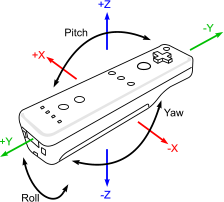
\includegraphics[width=0.4\textwidth]{docs/reports/Final Project Update/images/Wiimote_axes.png}
            \caption{\textbf{Wii Remote's Axes \cite{Axes}.}}
            \label{fig:Wii_axis}
        \end{figure}
        
        In order to achieve a functional connection with the Wii Remote, a custom driver made by Julian L\"{o}hr was used \cite{JulianLohr}. This driver, named HID Wiimote, is designed to allow the laptop to recognize the Wii remote's buttons and other sensors. The "HID" in the name refers to "human interface device," which is a general name for many devices that accept inputs from and provide feedback to a human user. With this driver, when the remote connects via Bluetooth, the LEDs stay lit and do not flash, meaning a connection has been completed successfully. The interface for this driver can be seen below. It allows the user to specify which accelerometers are recognized. It should be noted that there are only two accelerometers measured by this driver; the X- and Y-axis. These allow for the measurement of a tilt angle when the accelerometers detect portions of gravity in their axes, as normally the remote is oriented such that gravity is entirely in the Z-axis. These axes can be seen above in Figure \ref{fig:Wii_axis}. The battery level and a graphic corresponding to the LEDs on the remote are displayed in the top right.
        
        \begin{figure}[H]
            \centering
            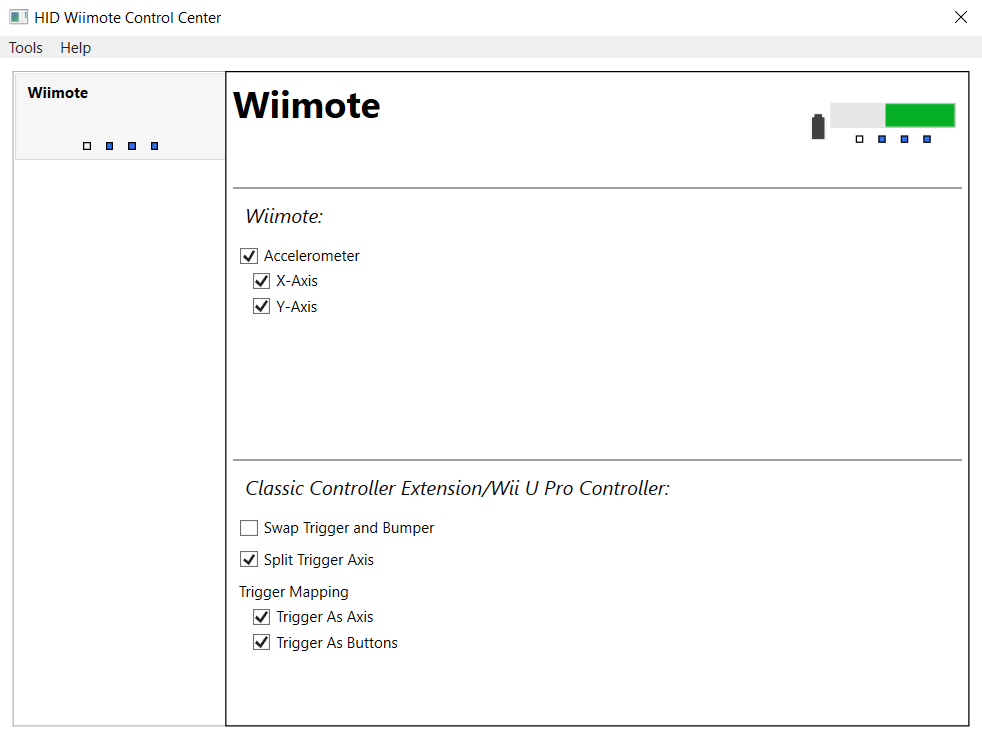
\includegraphics[width=0.7\textwidth]{docs/reports/Final Project Update/images/HID_GUI.PNG}
            \caption{\textbf{GUI of HID Driver.}}
            \label{fig:HID_driver}
        \end{figure}
        
        Now, the laptop can read the inputs from the Wii remote. Next, the inputs need to be mapped to specific functions. For this task, a software called JoyToKey was downloaded \cite{JoyToKey}. When a certain button is pressed or an accelerometer is activated, the corresponding output lights up as shown below. Then, the highlighted piece can be selected and configured to a key on the keyboard or the mouse itself. The GUI of JoyToKey can be seen below.
        
        \begin{figure}[H]
            \centering
            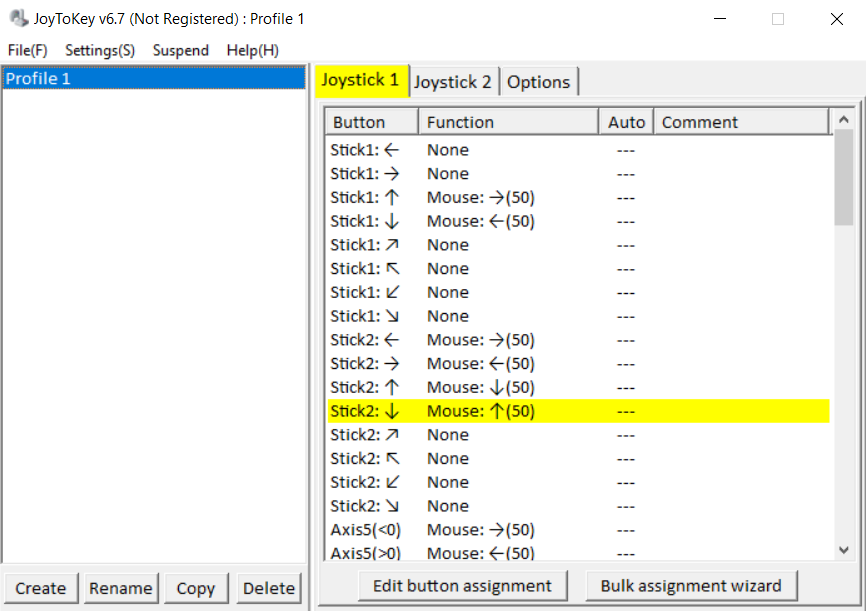
\includegraphics[width=0.7\textwidth]{docs/reports/Final Project Update/images/JoyToKey_GUI.PNG}
            \caption{\textbf{GUI of JoyToKey.}}
            \label{fig:JoyToKey}
        \end{figure}
        
        For the implementation of the Wii Remote controls, the mouse's inputs were mapped as accelerometer tilt measurements within the remote. To have the mouse go up and down, the remote was simply pitched up or down (about the X axis), and for the mouse to go side to side, the remote was rolled about its longitudinal (Y) axis. To initiate drawing, a mouse click was mapped as the 'A' button of the remote. Now the Wii remote is configured to be a magic wand that controls drones.


    % walk through code set up and implementation
    \subsection{Code Implementation}
    
        Figure \ref{fig:code_logic} describes the user interface logic with the program and considers the many cases in interaction when operating the drone. 
        
        \begin{figure}[H]
            \centering
            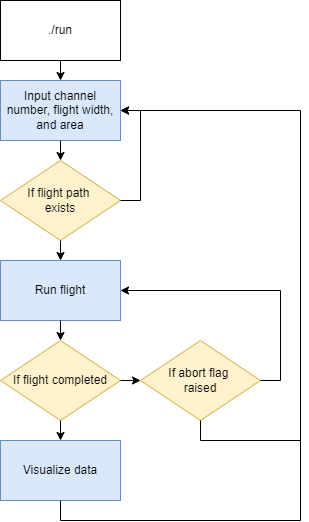
\includegraphics[width=0.4\textwidth]{docs/reports/Final Project Update/images/ae483_code_logic.png}
            \caption{\textbf{User interface logic.}}
            \label{fig:code_logic}
        \end{figure}
    
        \subsubsection{Python}
        
            % gui.py (Kenneth)
            The GUI allows for the abstractions of the Crazyflie client controller. Several control functions and the flight path canvas was implemented. One of the flight controller buttons is the Clear button that wipes the canvas and coordinate data. The Connect button establishes connection with the input channel number with the Crazyflie drone. The Run Flight button executes the drawn flight path scaled to the correct width of the flight zone. The Abort button suspends the flight and lands where the drone currently is.
            
            The main reason for implementation of the Abort button is the concern for safety. If the flight does not seem to go in the correct direction or is on a collision course with another object, the user can hit the abort the button to immediately land the drone. This was critical in the safety of our product, and utilized the threading concepts described previously. The abort flag is raised when the button is pressed, shutting down the function that moves the drone and lands it at the location that the button is pressed at. If the flight is aborted, the flight data will not be visualized and will be reset for the next flight.
            
            The canvas also allows for the user to use a mouse input as a way to draw the desired flight path. The canvas properly checks for cases that are out-of-bounds, and draws appropriately along the boundary of the canvas. The drawn pixels can be then converted to the world coordinates for the drone to fly in. 
            
            % client.py (Erika)
            The client code file was developed from the structure provided in AE483 lab, and altered to interact with the user interface. Notable changes begin with the channel specification, which is now set according to the user on the GUI end. A few additional functions were also created to interact with the drawn flight paths. The "flight" function is initialized when the user clicks the "Run Flight" button. The client calls on the "take\_off" function to begin flight, then moves the drone to a predetermined origin. Once at this origin, client.py takes in normalized pixel data as real-world move and smooth move commands. It commands these movements until the coordinate set is complete, then returns to the origin to power down.
             
            The client handles the flight paths and runs them according to the translated drawing that was received from the GUI. The class defined in this file is instantiated in the GUI.
            
            % flight data folder (Kenneth)
            For each flight, a folder is created to add the data after each flight. Utilizing the OS controls, a directory is created based on the date and time the flight concluded. Furthermore, the system takes a snapshot of the screen and saves that file in that same directory. The final data set that saves in that location are the JSON files for the flight data and a PNG file of the GUI interface. This will allow the user to return back to past flights if desired. 
            
            % main.py and run file (Kenneth)
            After creating the GUI and client interface classes, these files were integrated into the main function where everything can be run. The main file allows for the modularization of the different pieces of code and allows for the simplification of running code for the user. A run shell script was also created to abstract the file structure of the repository, and make it easier for the user to start up the GUI. 
        
        \subsubsection{Crazyflie Firmware}\label{crazyflie_firmware}
        % custom controller, og observer (Justin)
        
            The Crazyflie contains onboard firmware that interprets inputs from some source, be it a physical controller or pre-programmed commands, and turns them into commands for the Crazyflie's motors that move the drone from its current position and orientation towards a desired position and orientation. Custom firmware can be written and flashed to the drone to accomplish this kind of control. In particular, it is possible to implement a linear state feedback controller within the firmware that accepts desired position and orientation inputs and compares them to a state estimate that is iteratively updated with information from the drone's sensors.
            
            Within the AE 483 course, the implementation of a custom system was done in steps. First, the performance of the drone with the default controller and observer was characterized, and data was logged for offline processing. Next, a custom controller was implemented with the drone's default observer; i.e., the custom controller was paired with data extracted from the observer that would ordinarily send data to the the default controller. Finally, a custom observer was added to the custom firmware that eliminated the use of the default controller entirely.
            
            However, the performance of a fully-custom system with linear state feedback is lacking in comparison to the default system. This is discussed further in Section \ref{obsv_results}, though a key item of note is that there are only three controller and observer configurations that function in the current implementation. Namely, it is only possible to operate in fully default and fully custom modes (where both the controller and observer are the default or custom versions, respectively) as well as a mode that pairs a custom controller with the default observer. The inverse of the latter, trying to pair the \textit{default} controller with a \textit{custom} observer, does not work, and the drone instead overrides the custom observer with the default observer. This is likely due to a lack of logic in the code that would attempt to insert different observer data into the default controller-observer system.

\section{Results and Discussion}\label{results_discussion}

    \subsection{Implemented Features}
    
        % Summary (Erika)
        The primary feature which the group was successfully able to implement involved was the CopyCat mode. During the ideation phase, the group had come up with CopyCat, Live, and Spellcaster modes as different ways of commanding the drone. The latter two are elaborated upon in the Future Work section, but the group ran out of time to fully implement these modes. CopyCat is instead the mode featured through the bulk of the paper, wherein the user draws a coordinate set, and sends those coordinates to the drone to copy. This was a very involved process, from development of a graphical user interface, interfacing multiple files to command the drone, generating coordinates, and even plotting observer collected data post-flight.
        
        % Not on mac (Nintendo sux for proprietary software; can mention that drawing with mouse *does* still work on Mac tho) (George)
        With the implementation of the Wii remote, it was only successful while using Windows in the method outlined in Section \ref{WiiIMP}. The method outlined does not work with MacOS. Yet, if the Wii remote is not used, the path can still be drawn using any operating system if a mouse is used instead.
    
    % observer traced (Justin)
    \subsection{Observer Results}\label{obsv_results}
    
        %Custom observer less accurate and precise than default. Custom observer incompatible with default controller without potentially risky modification to default code.
        The three unique controller and observer configurations described in Section \ref{crazyflie_firmware} were flight-tested. The Tkinter Canvas was configured to plot the data recorded from the user input (as a black line) as well as the data logged from both observers after flight, with the default observer data in green and the custom observer data in blue. Figure \ref{fig:default_both} shows the drawn flight (a rough circle drawn counterclockwise) against the performance of the first configuration, the default controller and observer, as measured by the default observer. Data was not collected by the custom observer for this flight as it was not enabled. The performance appears to match the intended shape quite closely.
        
        \begin{figure}[H]
        \centering
        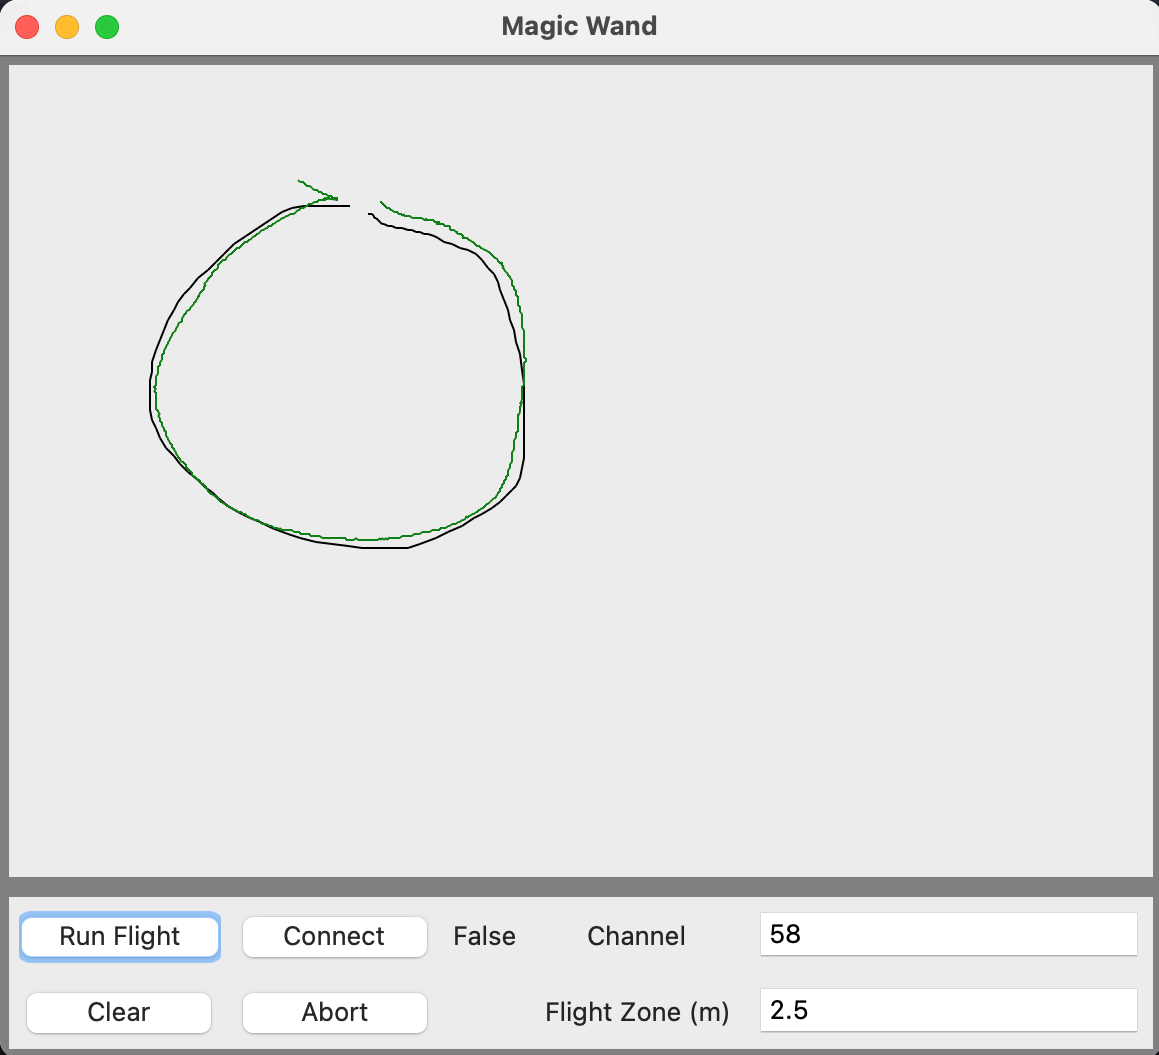
\includegraphics[width=0.6\textwidth]{docs/reports/Final Project Update/images/default_both.png}
        \captionsetup{width=0.6\textwidth}
        \caption{\textbf{GUI showing the drawn path (black) and performance of a fully default system according to the default observer position log (green).}}
        \label{fig:default_both}
        \end{figure}
        
        Figure \ref{fig:custom_ctrl_default_obsv} shows a different drawing (another counterclockwise circle) against the performance of the second configuration, a \textit{custom} controller with the default observer, again as measured by the default observer. In this configuration, the default observer's data is written as custom observer data to allow the custom controller to interpret it, hence why the blue line perfectly overlaps the green. Of note is that the controller seems to lag significantly, as the data collection starts when the drone \textit{should} be at the first position of the drawing, but the straight section after the beginning point of the blue circle shows that the drone was still translating from the origin at the expected start time. The wide gap at the end of the circle indicates the drone had not yet completed the shape at the expected end time. The "tail" of green that slightly extends beyond the blue shows that there may be notable delay in overwriting the custom observer measurements with default observer ones, perhaps contributing to a portion of the delay.
        
        \begin{figure}[H]
        \centering
        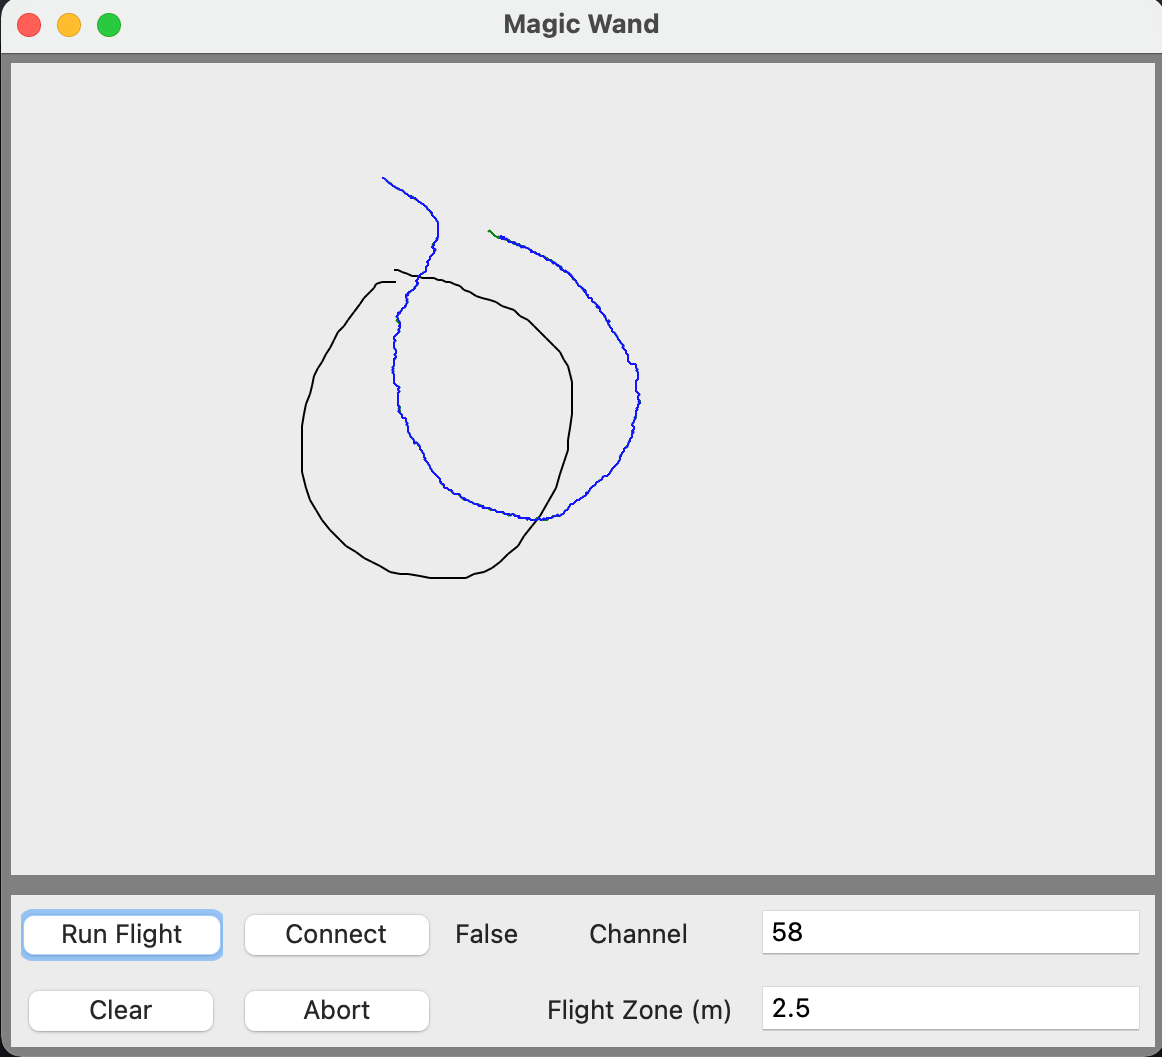
\includegraphics[width=0.6\textwidth]{docs/reports/Final Project Update/images/custom_ctrl_default_obsv.png}
        \captionsetup{width=0.6\textwidth}
        \caption{\textbf{GUI showing the drawn path (black) and performance of a custom controller and default observer system according to the default observer position log (blue).}}
        \label{fig:custom_ctrl_default_obsv}
        \end{figure}
        
        Figure \ref{fig:custom_both} shows yet another rough circle drawn counterclockwise, this time flown in the third configuration utilizing both the custom controller and observer. In this configuration, the default observer runs in the background, and its data is logged separately from the custom observer. The plotted paths from the observers show clear discrepancies in their respective position estimates. A video was taken of this flight, and it seems to indicate the default observer's measurements were closer to reality, though additional in-depth analysis of the video would be necessary to extract a real-world flight path to confirm this. In general, we have observed that the default observer plot appears closer to the actual flight path than the custom observer.
        
        \begin{figure}[H]
        \centering
        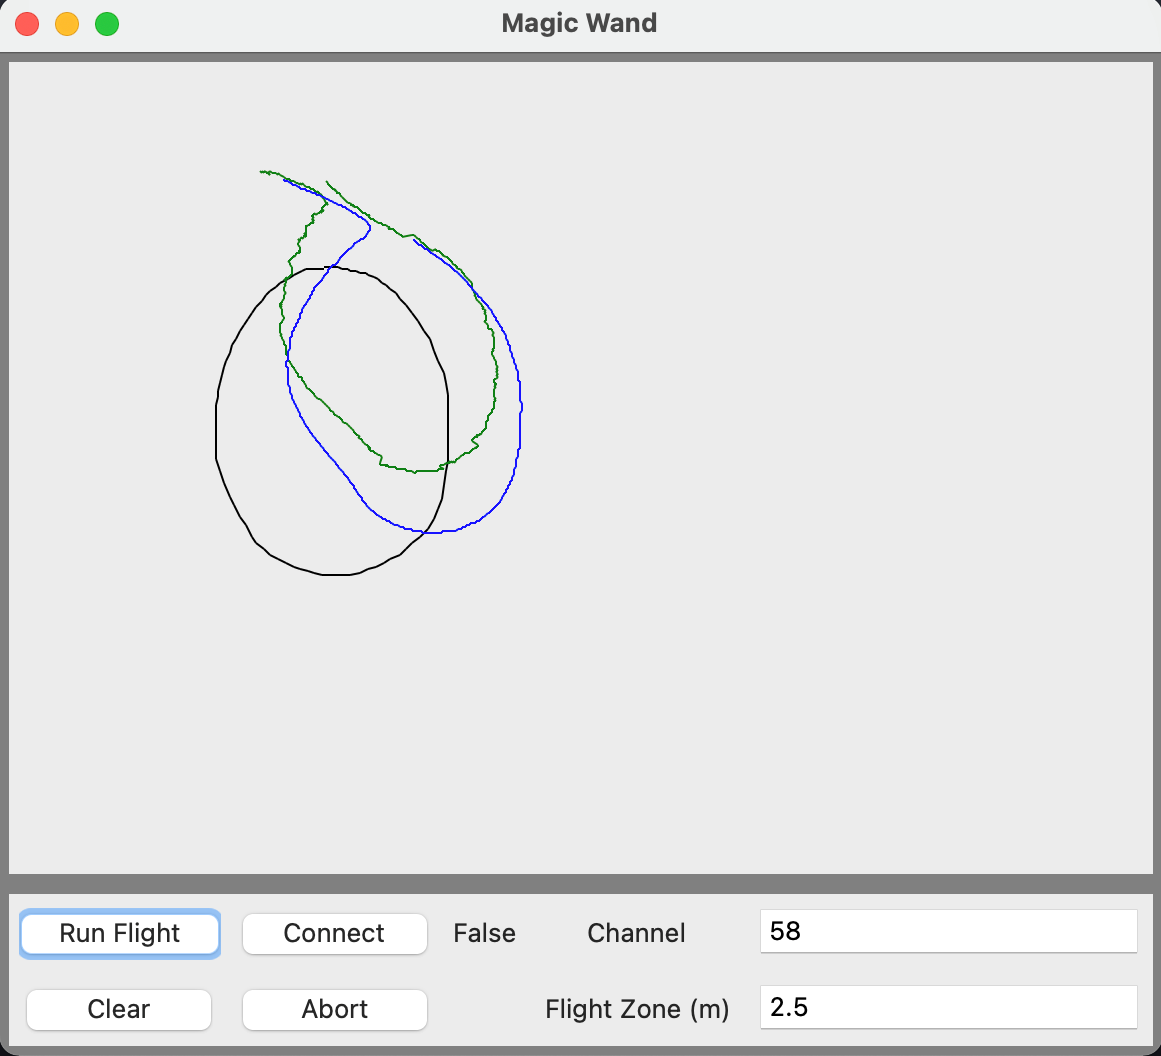
\includegraphics[width=0.6\textwidth]{docs/reports/Final Project Update/images/custom_both.png}
        \captionsetup{width=0.6\textwidth}
        \caption[width=0.6\textwidth]{\textbf{GUI showing the drawn path (black) and performance of a fully custom system according to both the default (green) and custom (blue) observer position logs.}}
        \label{fig:custom_both}
        \end{figure}
        
        Note that in each of Figures \ref{fig:default_both} through \ref{fig:custom_both} the shape was drawn with a trackpad on a device running macOS. This difference from using a Wii remote is not significant in evaluating the performance of the drone, as the Wii remote only serves as an alternative method of drawing.
        
        Among the three configurations, it is evident from data and real-world qualitative judgment that the default controller and observer combination displayed in Figure \ref{fig:default_both} provides the best performance to preserve the intended image. In the event one seeks to add an element of unpredictable character to their real-world flight path, the custom options remain available, provided the user has flashed the drone with the custom firmware and enables its use. This feature is not currently available in the GUI.
        
        In contrast to the observer-focused flights described previously, Figure \ref{fig:drawn_flight} instead shows a full-up test of the system with the default controller and observer. The intended shape was a skewed star in the top half of the drawing area. This was to ensure the overhead camera view in \ref{fig:real_flight} would capture the entirety of the flight. The imperfections in the drawn star demonstrate the difficulty of drawing accurately with the current accelerometer-only system, though with more practice one could likely improve with a learning curve similar to that of an Etch A Sketch.

        \begin{figure}[H]
        \centering
        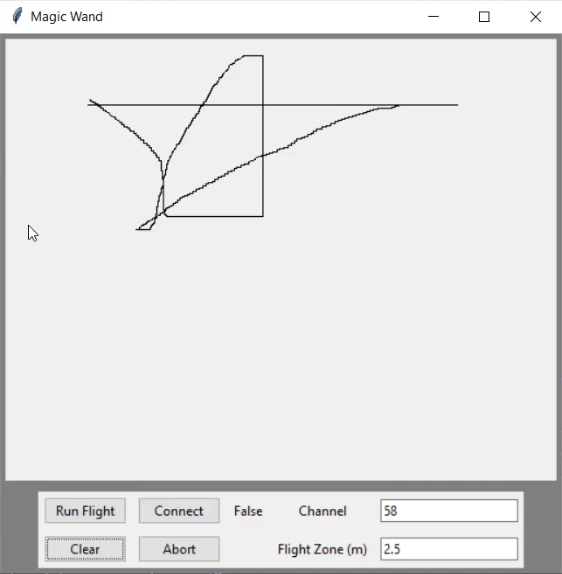
\includegraphics[width=0.6\textwidth]{docs/reports/Final Project Update/images/drawn_flight_path.PNG}
        \caption{\textbf{GUI with a sample flight drawn.}}
        \label{fig:drawn_flight}
        \end{figure}
        
        \begin{figure}[H]
        \centering
        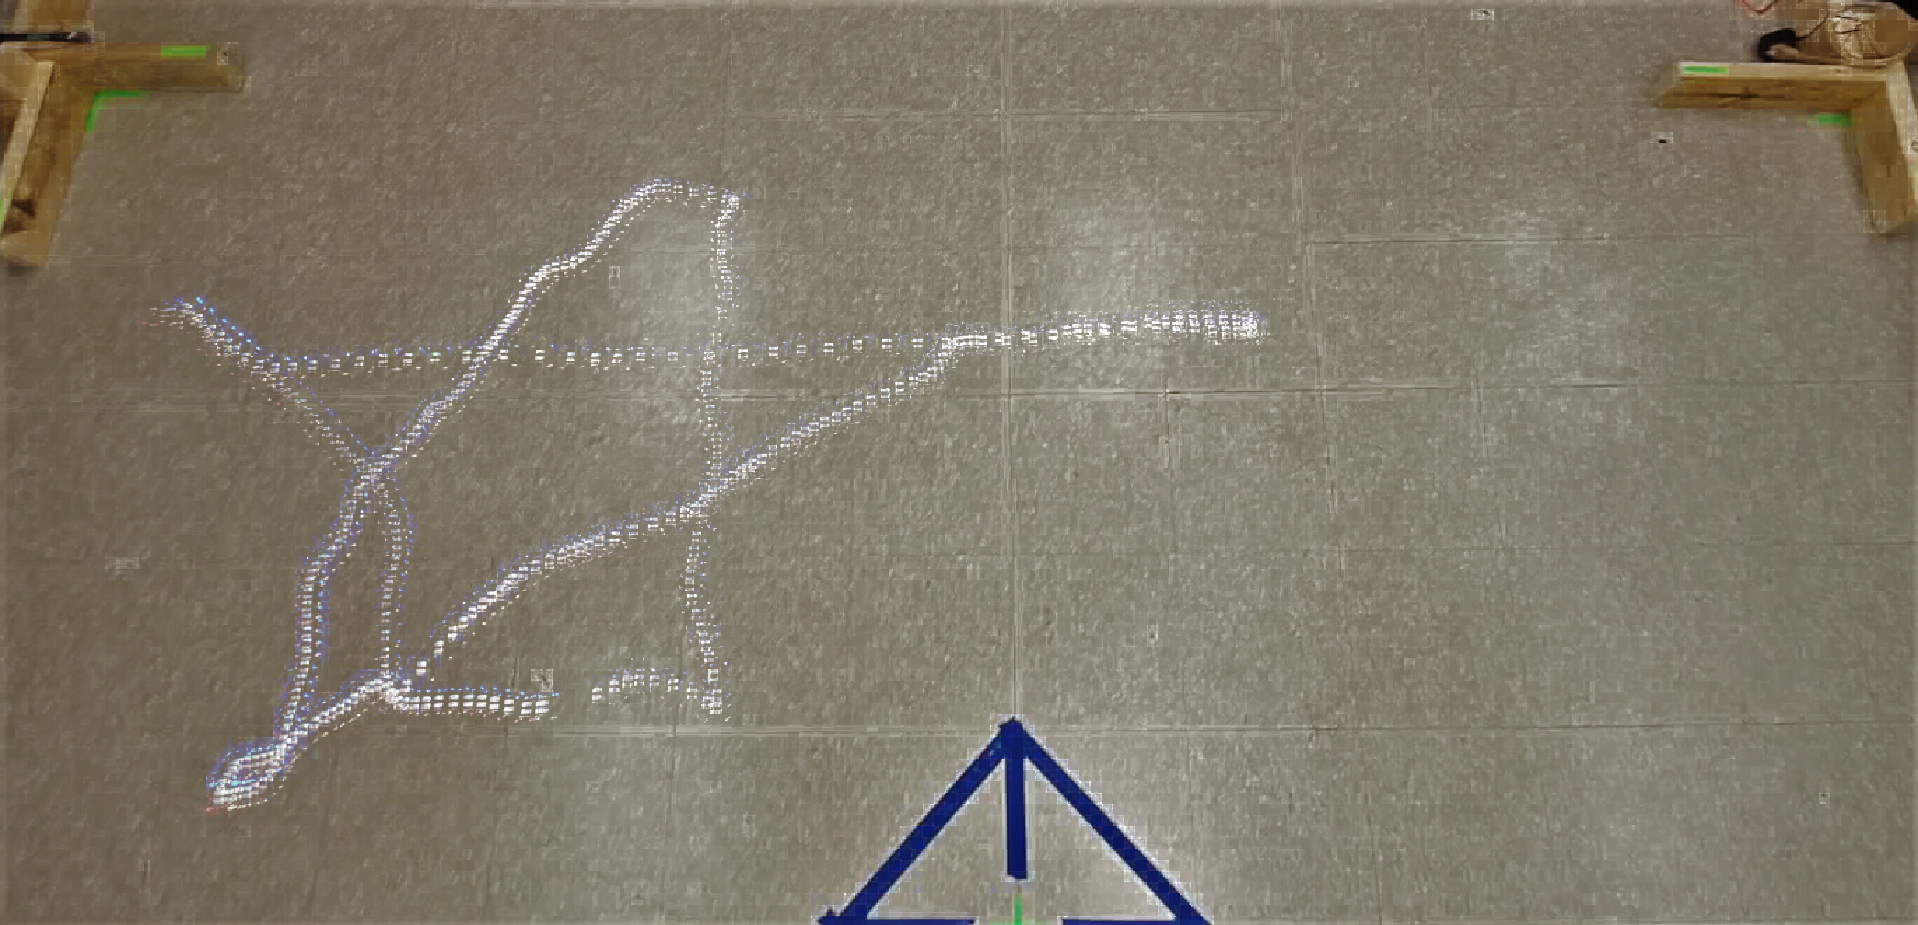
\includegraphics[width=0.6\textwidth]{docs/reports/Final Project Update/images/real_flight_path.png}
        \caption{\textbf{Real-world flight path of sample flight.}}
        \label{fig:real_flight}
        \end{figure}
        
        Figure \ref{fig:real_flight} was generated by taking every sixth frame of a 30 frames per second (FPS) video via an online video converter \cite{ezgif}, effectively producing a 5 FPS series of JPG images. These images were then used in Sequator, a star tracking program, to develop a "star trail" of the drone. Images were then edited to improve the contrast of this trail against the floor.
        
        The real-world overhead view bears a very strong resemblance to the shape drawn in the GUI. The speed with which one draws the figure in the GUI is deliberately coupled to the speed later flown by the drone, so for the quickly drawn horizontal line across the image, it is clear from the increased spacing that the drone was also moving more quickly. The complex twist at the lower left was drawn much more slowly and corresponds to a significantly higher number of frames per unit of distance traveled.
        
        Of note is that the lens used to record the original video was wide-angle, which causes distortion beyond the center of the frame. Furthermore, the drone was flying at 0.5 meters off the ground, while the camera was roughly 2.5 meters off the ground. This causes further apparent distortion and scaling. For these reasons, the image cannot be taken as a true representation of the real flight path. To image a real flight path, a series of cameras or a camera further away would help to eliminate these large effects.
        
        The method of light painting used in Figure \ref{fig:real_flight} technically works, though the discrete frames make it more useful as a technical tool for turning videos into images instead of a way to mimic high-quality long exposure images in darker environments, and heavy processing (necessary as a measure of efficiency) causes a notable drop in quality, namely via compression blockiness in the final image thanks to stacking JPG images of frames. In this particular image, 365 frames were stacked.
        
        A dark environment for proper light painting is infeasible with the configuration of the Crazyflie used, as the flow deck requires light to function properly. Typical long exposure methods in this configuration would have to make the drone contrast significantly with the ground by increasing its absorption or brightness. For the existing setup, the sensitivity of smartphone sensors could not be lowered sufficiently to create a long enough exposure without washing out the image.
        

    \subsection{Future Work}
    
        To further improve the functionality of this drone, a fully custom controller and observer should be implemented with modern controls to significantly decrease the computation power required on board. This will allow for increased and more complex applications of the drone with the available computing power. For example, combining this combining this software with observed positional states could increase the accuracy of the drone, especially after takeoff. Furthermore, collaborating with the long-exposure teams can allow for the user to draw a long exposure image on the GUI, which can be flown in the pattern to take a long exposure photo. Decreasing the computing power can open up these possibilities and further expand the capabilities of the drone. 
        
        The GUI can also be further improved with better functionalities. When the project was first started, some of the stretch-goals included implementing plane change radio buttons. This would allow for the user to change the 2D plane in which the drone flew in. Other functionalities include modes in which the user defines the flight path. One example would be a Spellcaster mode where a user would draw a pattern that corresponds to a specific flight path. If the pattern is close enough to a corresponding shape, the drone would fly in that specific pattern. Another example would be a Live mode where the drone directly responds to the location of the cursor in the drawing canvas. When the flight begins, the drone would move the location of the cursor and follow the cursor in real-time until the user commands the drone to land. These functionalities are rather complex but could be something that could be implemented to expand the capabilities of the project. 
        
        Finally finding a better solutions for the Wii remote seems more applicable for the project. IR sensors can help define a better location on the screen to allow for the user to draw more easily. Accelerometer data can get a sense of which direction to go, but the IR sensor will allow for a more accurate 2D location on the screen. Furthermore, due to the compatibility and legacy hardware issues arising with the Wii Remote, it may be beneficial to use a more up-to-date controller such as ones used in VR environments where the hand motions are tracked on the controller. This would allow for expanded use of the application, and more easily enable the "magic wand" effect with this interface. 

\section{Conclusion} % Justin
    We developed an intuitive graphical user interface utilizing object-oriented programming and interfaced a Nintendo Wii Remote with a Windows 10 computer to serve as mouse inputs that can be used to draw images. The GUI successfully interprets these drawings and converts them to flight paths that can be flown by the Bitcraze Crazyflie 2.0 drone. The performance of this system is acceptable, especially when the drone's built-in controller and observer are used. It is the judgment of the authors that there are several methods of advancing this concept further, and the current implementation would benefit from having further characterization of its performance via more rigorous data collection, perhaps enabling informed refinement of operations.
    
    Though the functionality does not strictly match the original intent to make the Wii Remote feel like a magic wand, the primary goal of developing the GUI and interfacing the Wii Remote were met. Simplification of the Wii Remote interface, particularly the elimination of the need for an infrared array, makes this system a simple and accessible way to interact with the Crazyflie.

\section{Acknowledgements}
    The authors thank their professor, Tim Bretl; their teaching assistant, Travis Zook; and their laboratory manager, Dan Block. We also thank teaching assistants Jacob Kraft and Max Kolarich for additional support and feedback.

\appendix

\section{Group Member Contributions} \label{apx:contributions}
    \begin{table}[H]
        \begin{center}
        \setstretch{1}
        \caption{\textbf{Contributions Table}}
        \begin{tabular}{ | p{2in} | p{4in}| } 
            \hline
            \textbf{Group Member} & \textbf{Contribution to Project} \\  \hline
            Erika Jarosch & Flight path code development and interfacing, co-authored Methods, Design, Results, Developed Jupyter Notebook\\ \hline
            George Petrov & Wii Remote implentation, documentation, authored Wii remote section on report\\ \hline
            Justin Roskamp & Interpreted real-world performance and configurations, co-authored Introduction, Design, Results, Conclusion   \\ \hline
            Kenneth Tochihara & GUI and client interface, repository management, documentation, co-authored code-implementation sections on report\\ \hline
        \end{tabular}
        \end{center}
    \end{table}

\section{Code Repository}
    GitHub Repository: \url{https://github.com/ktt3/ae483-magic-wand}


\setstretch{1}
\setlength{\parindent}{0pt}

\begin{thebibliography}{9}
    
\end{thebibliography}

\end{document}